%compile with pdflatex on papeeria

\documentclass[a4paper,12pt]{article}
\usepackage{fancyhdr}
%\usepackage{fancyheadings}
\usepackage[ngerman,german]{babel}
\usepackage{german}
\usepackage[utf8]{inputenc}
%\usepackage[latin1]{inputenc}
\usepackage[active]{srcltx}
%\usepackage{algorithm}
%\usepackage[noend]{algorithmic}
\usepackage{amsmath}
\usepackage{amssymb}
\usepackage{amsthm}
\usepackage{bbm}
\usepackage{enumerate}
\usepackage{graphicx}
\usepackage{ifthen}
\usepackage{listings}
\usepackage{enumitem}
%\usepackage{struktex}
\usepackage{hyperref}
\usepackage{tikz}
\usepackage{float}
\usepackage{subcaption}
\usepackage{array}
\captionsetup{compatibility=false}
\captionsetup[subfigure]{labelformat=empty}

\usepackage{pgfplots}
\usepgfplotslibrary{fillbetween}
%\usetikzlibrary{patterns}
\pgfplotsset{compat=1.15}
\usepackage{mathrsfs}
\usetikzlibrary{arrows}

\pgfplotsset{grid style={dashed,gray}}

\definecolor{kolorwykresu}{rgb}{0.07,0.04,0.56}

\definecolor{ccqqqq}{rgb}{0.8,0,0}

\pagenumbering{gobble}

\usepackage{siunitx}
\sisetup{per-mode = symbol, locale = DE}

\usepackage{tabularray}
\usepackage{multirow}
\usepackage{booktabs,tabularx}
\renewcommand\tabularxcolumn[1]{m{#1}}% for vertical centering text in X column

\newcolumntype{L}[1]{>{\raggedright\let\newline\\\arraybackslash\hspace{0pt}}m{#1}}
\newcolumntype{C}[1]{>{\centering\let\newline\\\arraybackslash\hspace{0pt}}m{#1}}
\newcolumntype{R}[1]{>{\raggedleft\let\newline\\\arraybackslash\hspace{0pt}}m{#1}}

\newcolumntype{Y}{>{\centering\arraybackslash}X}

%%%%%%%%%%%%%%%%%%%%%%%%%%%%%%%%%%%%%%%%%%%%%%%%%%%%%%
%%%%%%%%%%%%%% EDIT THIS PART %%%%%%%%%%%%%%%%%%%%%%%%
%%%%%%%%%%%%%%%%%%%%%%%%%%%%%%%%%%%%%%%%%%%%%%%%%%%%%%
\newcommand{\Fach}{2. Klausur aus der Mathematik (A)}
\newcommand{\Name}{}
\newcommand{\datum}{}
\newcommand{\Matrikelnummer}{}
\newcommand{\Semester}{Q12/2}
\newcommand{\Uebungsblatt}{} %  <-- UPDATE ME
%%%%%%%%%%%%%%%%%%%%%%%%%%%%%%%%%%%%%%%%%%%%%%%%%%%%%%
%%%%%%%%%%%%%%%%%%%%%%%%%%%%%%%%%%%%%%%%%%%%%%%%%%%%%%

\setlength{\parindent}{0em}
\topmargin -1.0cm
\oddsidemargin 0cm
\evensidemargin 0cm
\setlength{\textheight}{10.2in}
\setlength{\textwidth}{6.0in}
%\setlength{\footskip}{-1cm}

%%%%%%%%%%%%%%%
%% Aufgaben-COMMAND
\newcommand{\Aufgabe}[1]{
  {
  \vspace*{0.5cm}
  \textsf{\textbf{Aufgabe #1}}
  \vspace*{0.2cm}
  
  }
}
%%%%%%%%%%%%%%
\hypersetup{
    pdftitle={\Fach{}: Übungsblatt \Uebungsblatt{}},
    pdfauthor={\Name},
    pdfborder={0 0 0}
}

\lstset{ %
language=java,
basicstyle=\footnotesize\tt,
showtabs=false,
tabsize=2,
captionpos=b,
breaklines=true,
extendedchars=true,
showstringspaces=false,
flexiblecolumns=true,
}

\title{Übungsblatt \Uebungsblatt{}}
\author{\Name{}}

\begin{document}

\fancyhead{}
\fancyhead[C]{
\includegraphics[height=2.5cm]{lukasLogo.png}
\vspace{2cm}
}

\thispagestyle{fancy}
%\lhead{\sf \large \Fach{} \\ %\small \Name{} - \Matrikelnummer{}


\lhead{
%\vspace{1cm}
  \sf \LARGE \Fach{} %\small \Name{} - \Matrikelnummer{}
}
\rhead{\sf \Semester{}   \datum{}}

\vspace*{0.2cm}

\vspace{4cm}
Alle Lösungen müssen mit Nebenrechnungen und Begründungen nachvollziehbar sein!

%\rhead{\sf \Semester{} }
\vspace*{0.2cm}
%\begin{center}
%%\LARGE \sf \textbf{Übungsblatt \Uebungsblatt{}}
%\end{center}
%\vspace*{0.2cm}

%%%%%%%%%%%%%%%%%%%%%%%%%%%%%%%%%%%%%%%%%%%%%%%%%%%%%%
%% Insert your solutions here %%%%%%%%%%%%%%%%%%%%%%%%
%%%%%%%%%%%%%%%%%%%%%%%%%%%%%%%%%%%%%%%%%%%%%%%%%%%%%%

\vspace{1cm}
  Name: \underline{\hspace{7cm}}
%\draw[line width=1pt,color=ccqqqq,smooth,samples=100,domain=-6:7] plot(\x,{(1/12)*\x*\x+(1/3)*\x});
  \hfill
  Datum: \underline{\hspace{4cm}}

%\vspace{0,5cm}Die Rechenwege müssen nachvollziehbar sein!

%\vspace{1,5cm} {TEIL A} - ohne Hilfsmittel. Bearbeitungszeit 35 min.
\vspace {2cm}


\begin{center}
  \begin{tblr}{
      width=1\linewidth,
      colspec = {Q[c,6em]Q[c,4em]Q[c,4em]Q[c,4em]Q[c,4em]Q[c,4em]Q[c,4em]Q[c,4em]Q[c,6em]},
      rowspec = {Q[m]Q[m]Q[m]Q[m]Q[m]Q[m]Q[m]Q[m]Q[m]},
      colsep = 0mm,
      %row{1} = {2em,azure2,fg=white,font=\large\bfseries\sffamily},
      row{1} = {2em,font=\large\bfseries\sffamily},
      hlines, vlines,
    }
    \textbf{Aufgabe} & \textbf{1} & \textbf{2} & \textbf{3} & 
    \textbf{4} & \textbf{5} & \textbf{6} & \textbf{7} & \textbf{Gesamt} \\
    {Mögliche \\ Punkte} & {4} & {4} & {4} & 7 & 23 & 18 & 18 & 78 \\
    {Erreichte \\ Punkte} &  &  &  &  &  &  & &  \\
  \end{tblr}
\end{center}

\vspace{5cm}
\centerline{\huge\bfseries\sffamily Viel Erfolg !!!}

\newpage

\begin{center}
\vspace{0,5cm} {TEIL A} - ohne Hilfsmittel - Bearbeitungszeit 30 Minuten
\end{center}
\vspace {0,8cm}

ANALYSIS

\Aufgabe{1:} 
Berechnen Sie die unbestimmten Integrale:

\begin{enumerate}[label={\alph*)}]
  \item $ \int \frac{2x^2}{3x^3-3} dx $
    %\vspace{2,5cm}
  \item $ \int -4xe^{x^2+5} dx $
  %  \vspace{2,5cm}
  %\vspace{1cm}
\end{enumerate}
    \marginpar{4 BE}
%\begin{flushright}4 BE \end{flushright}
\Aufgabe{2:}
Welche Werte kann $ b \in R$ annehmen, damit folgende Gleichung stimmt? Begründen Sie kurz geometrisch und erklären Sie ausführlich!

 $ \int_ {-3}^{b} x^5 dx =0$
%\begin{flushright}4 BE \end{flushright}
    \marginpar{4 BE}
%\begin{flushright}Bitte wenden \end{flushright}

\vspace{2cm}
STOCHASTIK

\Aufgabe{3:}
Gegeben ist eine Zufallsgröße $X$, die die Werte $x_i = \{-2; 0; 2; 4\}$ annimmt.\\
Dem untenstehenden Histogramm kann man die Wahrscheinlichkeitswerte $P(X = x_i)$ entnehmen



\begin{figure}[h!]
  \centering
\begin{tikzpicture}[>=latex, line cap=round, line join=round,>=triangle 45]
\begin{axis}[
  %unit vector ratio=1 10,
  axis x line=center,
  axis y line=center,
  axis line style = thick,
  xtick align=inside,
  %extra x tick style={tick style={very thick}}
  xtick={-4,-2,0,2,4},
  ytick={0,0.1,0.2,0.3,0.4},
  xtick style=thick,
  ytick style=thick,
  xticklabels={,,},
  extra x ticks={-2,0,2,4},
  bar width=1cm,
  %xticklabel style={anchor=south west},
  %minor x tick num=1,
  %minor y tick num=1,
  %minor tick num = 1,
  x=1cm,    %größe der kästchen in x-richtung
  y=10cm,    %größe der kästchen in y-richtung
  xlabel={$x$},
  ylabel={$P(X=x)$},
  ymajorgrids=true,
  xlabel style={below right},
  ylabel style={below right},
  %xmajorgrids=true,
  xmin=-4,
  xmax=5,
  ymin=0,
  ymax=0.4]

\addplot[ybar,fill=blue,fill opacity=0.2] coordinates {
        (-2,0.2)
        (0,0.3)
        (4,0.2)
    };
\end{axis}
\end{tikzpicture}
\end{figure}

%\begin{figure}[h!]
%  \centering
%  \includegraphics[width=0.5\columnwidth]{210227_barChart_p.png}
%\end{figure}

Ergänzen Sie den zu $x_i=2$ gehörenden Wahrscheinlichkeitswert im Histogramm und ermitteln Sie näherungsweise den Erwartungswert der Zufallsgröße.

\newpage
GEOMETRIE

\Aufgabe{4:} 

Gegeben sind die Punkte $A (0|0|0)$ und $ C (5|3|4)$ sowie die Gerade

\[
       g: \vec{X} = \begin{pmatrix}10 \\ -3 \\-4 \end{pmatrix} 
                  + \lambda \begin{pmatrix}5 \\ -3 \\-4 \end{pmatrix}          
\] 
$(\lambda \in \mathbb{R})$

\begin{enumerate}[label={\alph*)}]
\item Zeigen Sie, dass $ g$  eine Mittelsenkrechte von $A$ und $C$ ist.
\item  Die Punkte A und C bilden zusammen mit zwei auf g liegenden Punkten das Quadrat
 $ABCD$. Bestimmen Sie die Koordinaten von B und D.
\end{enumerate}
%\begin{flushright}7 BE \end{flushright}
    \marginpar{7 BE}

\vspace {0,5cm}


\newpage


\begin{center}
\vspace{0,5cm} {TEIL B} - mit Hilfsmittel - Bearbeitungszeit 150 Minuten
\end{center}
\vspace {0,2cm}


\vspace {1,5cm}
ANALYSIS

\Aufgabe{5:}
Gegeben ist die Funktion $f: x\mapsto \frac{1-x}{1+x}$ mit dem Definitionsbereich $D_f = \mathbb{R}\setminus\{-1\}$. Der Graph von $f$ wird mit $G_f$, bezeichnet.

\begin{enumerate}[label={\alph*)}]
  \item Untersuchen Sie das Verhalten von $f$ an der Rändern des Definitionsbereichs und geben Sie die Gleichungen der Asymptoten von $G_f$ an.
    \marginpar{3 BE}
  \item Die Terme der gebrochen-rationalen Funktionen $g$ und $h$ haben den gleichen Zähler wie $f(x)$, aber jeweils einer anderen Nenner. Geben Sie je einen möglichen Funktionsterm für $g$ und $h$ an, sodass (bei jeweils maximalem Definitionsbereich) gilt:\\
  - Der Graph von $g$ hat keine senkrechte Asymptote.\\
  - Die Funktion $h$ hat an der Stelle $x = -1$ eine Polstelle ohne Vorzeichenwechsel.
    \marginpar{2 BE}
  \item Geben Sie die Koordinaten der Achsenschnittpunkte von $G_f$ an und untersuchen Sie das Monotonieverhalten von $G_f$. 
    \marginpar{4 BE}
  \item Zeichnen Sie $G_f$ unter Verwendung der bisherigen Ergebnisse in ein geeignetes Koordinatensystem ein.
    \marginpar{2 BE}

  \item Begründen Sie, dass die Funktion $f$ umkehrbar ist. Bestimmen Sie den Term der Umkehrfunktion von $f$.\\
  Was lässt sich aus dem Ergebnis hinsichtlich der Symmetrie von $G_f$ folgern?
    \marginpar{4 BE}

\item Bestätigen Sie, dass die Funktion $F: x\mapsto -x+2 \ln (x + 1); x \in \left]-1; \infty \right[$, eine Stammfunktion der Funktion $f^*: x\mapsto f(x); D_{f^*}= \left]-1; \infty \right[$, ist. 
    \marginpar{2 BE}
\\
\\
\newpage
    Die Ergebnisse der Teilaufgaben a) bis f) können im Folgenden verwendet werden.\\
\\

Eine Kugel $A$ der Masse 1 kg bewegt sich nach rechts und stoßt mit der Geschwindigkeit $1\frac{m}{s}$ elastisch und zentral auf eine gleich große ruhende Kugel B.

\begin{tikzpicture}
  \shade[ball color = gray!40, opacity = 0.4] (0,0) circle (1.5cm);
  %\draw (0,0) circle (2cm);
  \draw[->] (0,0 ) -- node[above]{$$} (2,0);

  \node[align=center] at (0,-2) {Kugel A};

  \shade[ball color = gray!40, opacity = 0.4] (6,0) circle (1.5cm);
  \node[align=center] at (6,-2) {Kugel B};

\end{tikzpicture}

    Die Maßzahl der Geschwindigkeit der Kugel $A$ in $\frac{m}{s}$ unmittelbar nach dem Zusammenstoß wird durch die Funktion $v: m\mapsto \frac{1-m}{1+m}$ mit $m \in \mathbb{R}$ beschrieben, wobei $m$ für die Maßzahl der Masse der Kugel $B$ in kg steht.\\
Zu einer Bewegung nach rechts gehören positive Geschwindigkeiten, zu einer Bewegung nach links negative Geschwindigkeiten.

\item Berechnen Sie, mit welcher Geschwindigkeit sich die Kugel $A$ unmittelbar nach dem Stoß bewegt, wenn die Masse der Kugel $B$ 0,6 kg beträgt.\\
  Geben Sie die Grenzwerte der Funktion $v$ für $m \rightarrow 0^+$ sowie $m \rightarrow +\infty$ an und machen Sie für diese beiden Grenzfälle jeweils den Bewegungsablauf der Kugel $A$ im Sachzusammenhang plausibel.
    \marginpar{3 BE}

\item Ermitteln Sie, für welche Werte von $m$ sich die Kugel $A$ unmittelbar nach dem Stoß nach rechts bewegt.\\
  Berechnen Sie, für welchen Wert von $m$ sich die Kugel $A$ unmittelbar nach dem Stoß mit $\num{0,9} \frac{m}{s}$ nach links bewegt.
    \marginpar{3 BE}
\end{enumerate}

\newpage
%\addtolength{\voffset}{-2cm}

STOCHASTIK

\Aufgabe{6:} 

Ein älteres Kopiergerät liefert brauchbare und unbrauchbare Kopien. Die Wahrscheinlichkeit, eine Kopie unbrauchbar ist, beträgt 15\% (Ausschussquote). Das Fertigen von Kopien soll als Bernoulli-Kette angesehen werden.

\begin{enumerate}[label={\alph*)}]
  \item Es werden 15 Kopien gefertigt. Ermitteln Sie die Wahrscheinlichkeiten der Ereignisse\\
    A: Mindestens 2, aber weniger als 6 Kopien sind unbrauchbar.\\
    B: Genau 3 Kopien sind unbrauchbar und diese folgen unmittelbar hintereinander.
    \marginpar{4 BE}
  \item Von einem einseitigen Rundschreiben werden 85 brauchbare Kopien benötigt. Da die Aus schussquote von 15\% bekannt ist, werden zur Sicherheit 100 Kopien angefertigt. Mit welcher Wahrscheinlichkeit erhält man trotzdem weniger brauchbare Kopien als benötigt?
    \marginpar{2 BE}
  \item Eine Mathelehrerin fertigt 50 Kopien (wieder mehr als eigentlich nötig sind) und schimpft: ,,Die Wahrscheinlichkeit dafür, dass ich genau so viele brauchbare Kopien erhalte wie ich benötige, liegt so immerhin bei über 10\%.'' Wie viele brauchbare Kopien könnte sie benötigen? Nennen Sie alle Möglichkeiten.
    \marginpar{2 BE}
  \item Ein Lehrer fertigt 28 Kopien. Mit welcher Wahrscheinlichkeit sind genau 4 davon unbrauchbar?
    \marginpar{2 BE}
  \item Der Lehrer geht mit 28 Kopien, von denen 4 unbrauchbar sind, in seinen Kurs, und vergisst, die unbrauchbaren Kopien auszusortieren. Er teilt zufällig je eine Kopie an seine 20 Schüler aus Mit welcher Wahrscheinlichkeit erhalten genau zwei Schüler eine unbrauchbare Kopie?
    \marginpar{2 BE}
  \item Ein Handwerker untersucht die Fehler beim Kopieren. Wie viele Kopien muss er mindestens machen, damit mit einer Wahrscheinlichkeit von mindestens 99\% mindestens eine unbrauchbare Kopie auftritt? 
    \marginpar{3 BE}
  \item Nach Abschluss der Reparaturarbeiten beträgt die Ausschussquote 5\%. Die Sekretärin fertigt 200 Kopien. Mit welcher Wahrscheinlichkeit weicht die Anzahl unbrauchbarer Kopien um höchstens eine Standardabweichung vom Erwartungswert ab?\\
    \marginpar{3 BE}
\end{enumerate}

\newpage
\addtolength{\voffset}{-2cm}
GEOMETRIE

\Aufgabe{7:} 
Die folgende Abbildung zeigt modellhaft eine Tribüne, die auf einer horizontalen Fläche steht.

\begin{figure}[h!]
  \begin{center}
    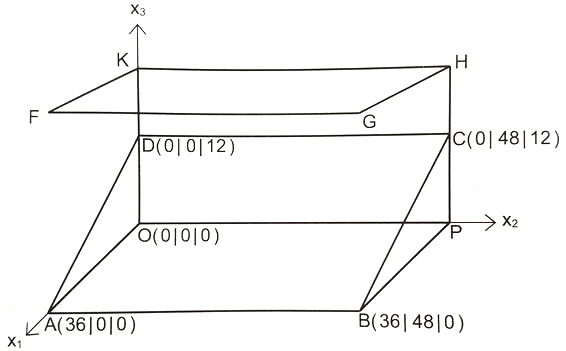
\includegraphics[width=0.5\linewidth]{tribüne.jpg}
    %\caption{A boat.}
    %\label{fig:boat1}
  \end{center}
\end{figure}


\enlargethispage{2cm}

Dabei beschreibt das Rechteck ABCD mit
  $A (36|0|0)$, $ B (36|48|0)$, $C (0|48|12)$ und $ D (0|0|12) $
die Nutzfläche der Tribüne. Das Rechteck ABPO stellt die Grundfläche der Tribüne dar, das
Rechteck FGHK beschreibt die Dachfläche der Tribüne. Die Eckpunkte der Dachfläche liegen
senkrecht über den entsprechenden Eckpunkten der Grundfläche.
Die $x_1x_2 $  Ebene stellt den Erdboden dar. Die $ x_1$ – Achse zeigt nach Süden, die $x_2$ – Achse nach
Osten. Eine Längeneinheit im Koordinatensystem entspricht 1m in der Realität, d.h. die Tribüne ist
48m breit. Die Materialstärke ist bei den Rechnungen zu vernachlässigen.
\begin{enumerate}[label={\alph*)}]
\item  Bestimmen Sie eine Gleichung der Ebene N, in der das Rechteck ABCD liegt, in
Normalenform. (zur Kontrolle:$ x_1 + 3x_3 = 36 $)
    \marginpar{4 BE}
\item Berechnen Sie die Größe des Neigungswinkels der Nutzfläche gegen die Horizontale.
    \marginpar{3 BE}
\item Die Dachfläche liegt im Modell in der Ebene $E: x_1 - 6x_3 + 96 = 0.$
Ermitteln Sie die Koordinaten des Punktes G, der im Modell einen Dachflächeneckpunkt
darstellt und senkrecht über dem Punkt B liegt. (zur Kontrolle: $G (36|48|22)$)
    \marginpar{4 BE}
\item Zur Installation von Lautsprechern soll eine Metallstange so an der Tribüne befestigt
werden, dass sie an dem Punkt beginnt, der im Modell durch den Punkt $G (36|48|22)$  beschrieben wird
und an der Nutzflächenkante endet, die im Modell durch die Strecke [BC] dargestellt wird.
Aus Kostengründen soll die Stange so kurz wie möglich sein. Untersuchen Sie, ob eine 20m
lange Stange ausreicht.
    \marginpar{4 BE}
\item An der Dachflächenkante Richtung Spielstätte, im Modell dargestellt durch die Strecke
[FG], soll eine Regenrinne abgehängt werden. Ein Befestigungspunkt R liegt 2 cm
unterhalb von G. Die Lage des zweiten Befestigungspunktes wird unterhalb von F so
gewählt, dass die Regenrinne auf einer horizontalen Länge von 2 m um 2 mm abfällt. Das
Wasser soll dabei Richtung Westen abfließen. Geben Sie eine Gleichung der Geraden h an,
die den Verlauf der Regenrinne zwischen den Befestigungspunkten im Modell beschreibt.
    \marginpar{3 BE}
\end{enumerate}
\vspace{0,8cm}


\centerline{Viel Erfolg}

\end{document}
